\documentclass[../thesis.tex]{subfiles}

\begin{document}

\chapter{Prescriptive Analytics to Support Capacity Planning for Frail and Elderly Patients}\label{chp:presciptive}

%\chapter{Deterministic and Stochastic (Mixed) Integer Programming for Frail and Elderly Patients}\label{chp:presciptive}
\section{Introduction}

Data analytics is categorised into three main \textcolor{blue}{paradigms}, each with a correspondingly varying degree \textcolor{blue}{of complexity}: descriptive analytics, predictive analytics and prescriptive analytics. In both industry and healthcare analytics, the first two stages have been extensively studied and documented. The third, and most complex \textcolor{blue}{\cite{Hertog2016}} to perform is prescriptive analytics which seeks to address the questions of `What should I do?' and `Why should I do this?'. Prescriptive analytics eliminates the risk by bridging the gap between the data that an organisation has and the consequences of implementing new policy. Decision-makers can gain a deeper grasp of how to seize an opportunity or alleviate a problem in the future as a result. Literature reviews in this area of OR have only recently been published, making it a relatively new and developing discipline \cite{Islam2018,Lopes2020,Lepenioti2019}. In all three articles, the application of prescriptive analytics is discussed, with Lopes et al. \cite{Lopes2020} arguing that successful optimisation of current healthcare resources will in turn decrease existing waiting lines and allow a greater ability to treat individuals in need effectively. Islam et al. \cite{Islam2018} discovered that just 9\% of the publications analysed within their review focused on prescriptive analytics, demonstrating that this a new and emerging area of healthcare research.

%Both articles examine the possibilities for the application of prescriptive analytics with Lopes et al. \cite{Lopes2020} arguing that successful optimisation of current healthcare resources will in turn shorten existing waiting lines and allow a greater ability to provide treatment effectively to individuals in need. 

\begin{description}
\item[\textcolor{red}{Research Aim}] - This chapter will present the underlying theory in order to address two of the research's objectives: `How can deterministic and stochastic models be used to successfully model hospital services?' and `How best can specialties be organised among a network of hospitals to ensure staffing and bed costs are minimised?'.
\end{description}

This research project was funded and carried out in collaboration with Clinical Futures in ABUHB \cite{UniAneurinBevanHealthBoard2018}. The organisation are restructuring and organising hospital services in order to improve patient care. One of their primary issues is determining the number of beds required to meet the existing demands for their frail and elderly population. Wards in the UK have minimal staff to patient ratios that are typically computed based on ward bed counts. We can extend this model to incorporate workforce planning and the number of nursing staff the health board should have available by determining the number of beds for each speciality within each hospital to fulfil demand.

Two-stage stochastic programming lends itself well to this type of problem, because bed numbers and staff must be planned in advance. Only when the demand for both elective and emergency patients is known can it be established whether sufficient beds and staff have been planned. If not, additional beds and staff are needed to meet this demand safely. Because this is not planned in advance, there are typically additional charges, such as relocating patients to different hospitals, opening new wards, and contacting agency and bank personnel. Before deciding on two-stage stochastic modelling for this project, a variety of other stochastic models were studied. Following are the justifications provided for their exclusion:

\begin{itemize}
    \item \textcolor{blue}{\textbf{Markov Models} - Markov models are based on a set of states, with the underlying theory that the future states depend only on the current states, not on the events that have occurred prior to this. In healthcare bed modelling, historical data is used to plan the number of beds, due to either seasonal changes, or day of the week changes. One limitation of these models is the difficulty to model a large number of states \cite{Carta2020}. Since a network of hospitals and a range of specialties were going to be considered, this would create a large and computationally heavy Markov model.}
    % \item\textcolor{blue}{\textbf{Simulation} - }
    \item \textcolor{blue}{\textbf{Queueing Theory} - Queueing theory concerns the study of waiting lines \cite{Shortle2017}. It translates customer arrival characteristics and service patterns into measures of waiting experienced by the customer. We do not, however, know the characteristics of customer arrival because we concentrate on patients who have been admitted rather than how patients entered the system.}
    \item \textcolor{blue}{\textbf{Newsvendor Models} - Newsvendor Models determine the quantity of products to invest in before the demand is known, with the goal of selecting the investment amount in the best way to reduce waste \cite{Silver2016}. In the ABUHB scenario, having the option to add more `stock' (beds and nursing staff), if demand cannot be met would make the situation more practical for the healthcare industry because patients who require admission would not be turned away. Additionally, with inpatients in hospitals, beds are frequently occupied for longer than one day, so the stock would not return to zero as it does with standard Newsvendor models, which have a day-end stock value of zero.}
\end{itemize}

To identify the most cost-effective way to arrange specialised beds and nurses in hospitals, deterministic and two-stage stochastic modelling can be used. \textcolor{blue}{The health board has historically planned the number of beds and nurses on staff using averages (deterministic). Due to emergency admissions, cancellations, and fluctuating admission LOS's, bed planning can be challenging. Stochastic modelling can help overcome this challenge and provide more informed outcomes. We present a two-stage stochastic model that takes system unpredictability into consideration when scheduling nursing staff and beds.} Similar to the chapter on predictive analytics, a worked example will be provided to show how each method operates. Recall the worked example from Chapter \ref{chp:predictive}, where fifteen patients with various attributes attended one of two hospitals in South East Wales. Following is a table of these patients:

\begin{table}[h!]
    \centering
    \begin{adjustbox}{width=\columnwidth}
    \begin{tabular}{cccccccc}\toprule
       \textbf{Patient Number}  & \textbf{Age} & \textbf{Hospital} & \textbf{LOS} & \textbf{Specialty} &\textbf{Admission Method} & \textbf{Admission Source} & \textbf{Frailty Source} \\\midrule
        Patient 1 & 95 & RGH & 5 & COTE & Emergency & Own Home & 3 \\ 
        Patient 2 & 82 & RGH & 3 & COTE & Emergency & Own Home & 2 \\
        Patient 3 & 89 & RGH & 4& T\&O & Emergency & Own Home & 2 \\
        Patient 4 & 87 & RGH & 4 & T\&O & Elective & Own Home & 2 \\
        Patient 5 & 85 & NHH & 3 & COTE & Elective & Transferred & 1 \\
        Patient 6 & 76 & NHH & 1 & COTE & Elective & Transferred & 1\\
        Patient 7 & 71 & NHH & 1 & T\&O & Emergency & Transferred & 1 \\
        Patient 8 & 96 & RGH & 5 & T\&O & Emergency & Own Home & 3 \\
        Patient 9 & 70 & NHH & 1 & COTE & Emergency & Transferred & 1\\
        Patient 10 & 67 & NHH & 1 & T\&O & Elective & Own Home & 1\\
        Patient 11 & 89 & RGH & 4 & COTE & Elective & Transferred & 3\\
        Patient 12 & 70 & NHH & 1 & COTE & Elective & Own Home & 2\\
        Patient 13 & 75 & NHH & 4 & T\&O & Elective & Transferred & 3\\
        Patient 14 & 72 & NHH & 2 & COTE & Elective & Transferred & 3\\
        Patient 15 & 87 & RGH & 5 & COTE & Emergency & Own Home & 2\\\bottomrule
    \end{tabular}
    \end{adjustbox}
    \caption{Worked Example Patient Data - 15 Patients}
    %\label{tab:WETableExtended}
\end{table}


% \[
% \begin{blockarray}{ccccccccc}
%     &\matindex{Age} & \matindex{Hospital} & \matindex{LOS} & \matindex{Specialty} & \matindex{Admission Method}&\matindex{Admission Source} & \matindex{Frailty Level}\\
%     \begin{block}{c(cccccccc)}
%      \matindex{Patient 1}&  95 & RGH & 5& COTE & Emergency & \text{\textit{Own Home}} & 3\\
%      \matindex{Patient 2}&  82 & RGH & 3& COTE& Emergency& \text{\textit{Own Home}} & 2\\
%      \matindex{Patient 3}&  89 & RGH & 4 & T\&O & Emergency& \text{\textit{Own Home}} & 2 \\
%      \matindex{Patient 4}&  87 & RGH & 4 & T\&O& Elective & \text{\textit{Own Home}} & 2\\
%      \matindex{Patient 5}&  85 & NHH & 3 & COTE & Elective& \text{\textit{Transferred}} &1 \\
%      \matindex{Patient 6}&  76 & NHH & 1 & COTE & Elective& \text{\textit{Transferred}} & 1\\
%      \matindex{Patient 7}&  71 & NHH & 1 & T\&O& Emergency& \text{\textit{Transferred}}& 1\\
%      \matindex{Patient 8}&  96 & RGH & 5 & T\&O& Emergency& \text{\textit{Own Home}} & 3\\
%      \matindex{Patient 9}&  70 & NHH & 1 & COTE& Emergency & \text{\textit{Transferred}}&1\\
%      \matindex{Patient 10}&  67 & NHH & 1 & T\&O & Elective & \text{\textit{Own Home}} &1\\
%           \matindex{Patient 11}&  89 & RGH & 4& COTE & Elective & Transferred & 3\\
% \matindex{Patient 12} &	70 &	NHH &	1 &	COTE &	Elective &	\text{\textit{Own Home}}&	2\\
% \matindex{Patient 13} &75 &	NHH &	4 &	T\&O &	Elective&	Transferred&	3\\
% \matindex{Patient 14}&	72&	NHH&	2 &	COTE&	Elective &	Transferred &	3\\
% \matindex{Patient 15} &	87 &	RGH &	5&	COTE &	Emergency &	\text{\textit{Own Home}} &	2\\
%     \end{block}
%   \end{blockarray}
% \]

\textcolor{blue}{To ascertain whether there is a benefit to employing the two-stage stochastic model as opposed to the deterministic counterpart, the work by Maggioni and Wallace \cite{Maggioni2010} will be utilised. Within their paper, the authors discuss the quality of the expected value solution in stochastic programming and apply their models to four case studies: Single-sink transportation problem, production problem, location routing (network design) problem and a mobile ad-hoc network problem. The authors outline four experiments in which they determine the factors that contributed to the expected value solution. \textcolor{blue}{Their work will be expanded upon by applying the theory to a different case study of bed and resource planning. Three of the four experiments (due to relevancy), will be applied to healthcare services for elderly and frail patients. This in turn will determine the factors that contribute to the expected value solution.} 

Using the deterministic and two-stage stochastic optimisation techniques this chapter will examine how to effectively organise bed and staffing resources for hospitals. With these models, a user can modify the model to account for the number of hospitals and medical specialisations involved in their particular case. The remainder of the chapter is set out as follows:  The prescriptive methods employed in this research and their current use in healthcare are covered in Section \ref{sec:prescriptive}. The development of the deterministic model is shown in Section \ref{sec:DeterministicModel}, whereas Section \ref{sec:twostagestochasticmodel} provides a similar analysis using a two-stage stochastic model. The two approaches are combined in Section \ref{sec:evalofmeasures} to assess the performance of the stochastic or deterministic models. Throughout the chapter, a condensed practical example will be given.

\section{Prescriptive Techniques} \label{sec:prescriptive}

Prescriptive analytics is the process of using data and applying it to determine an optimal course of action. It builds upon the work of descriptive and predictive analytics and can broken down into three approaches:
\begin{itemize}
    \item Bridging the gap between potential and recommend outcomes
    \item Turning data into practical strategies
    \item Providing a clear path forward even with messy data
\end{itemize}

Prescriptive analytics incorporates large amounts of structured and unstructured data to determine the consequences of making decisions and how the future would be impacted. Furthermore, it can measure the repercussions of a decision based on different possible future scenarios. Organisations will increasingly need to find ways to take advantage of their data, especially as it continues to grow \hl{REFERENCE THIS ORE REMOVE}. Prescriptive analytics benefits organisations by allowing them to get the most out of their data and automate key procedures.

Table \ref{tab:PrescriptiveMethods}, consists of a collection of prescriptive analytics methods and associated healthcare papers.
\begin{table}[h!]
    \centering\scalebox{0.8}{
    \begin{tabular}{ll}\toprule
        \textbf{Method} & \textbf{Healthcare Examples} \\\midrule
        Heuristics & Facility Location Problem \cite{Kady2017,Kim2013}, Routing Problem \cite{Grenouilleau,Liu2013,Valipour2013} \\
        \textcolor{blue}{Markov Methods} &\textcolor{blue}{Health Management \cite{McClean2006,Sanchez2007}, Readmissions \cite{Bartolomeo2008,BenAssuli2020,Verma2018}, Scheduling \cite{Ala2022,Kolesar1970}} \\
        Optimisation & Outpatient appointments \cite{Perez2013,Srinivas2018,Zacharias2013}, Inventory Management \cite{Galli2020,Pardede2019} \\
        \textcolor{blue}{Queueing Theory} & \textcolor{blue}{Patient \& Optimise Performance \cite{Day2010, Komashie2015}, Hospital Satisfaction \cite{Ameh2013,Komashie2015},}\\
       & \textcolor{blue}{Waiting Times \cite{Cochran2009,Joustra2009,Siddharthan1996}}\\
        Reinforcement Learning & Resource Allocation \cite{Schuetz2012}, Drug Development \cite{Olivecrona2017,Popova2018,Serrano2018},  \\& Health Management \cite{Baniya2017,YomTov2017} \\
        Simulation & Capacity planning \cite{Carmen2015,Ponis2013,Williams}, Patient Flow \cite{Weng2011,Wong2011}, Scheduling \cite{Komashie2008} \\
        \textcolor{blue}{Soft OR} & \textcolor{blue}{Emergency Care \cite{Kuo2020,Newell2017,Widmer2017}, Telehealth Intervention \cite{Bashshur2016,Carter2018,Gordon2020}, } \\ &{ Patient Discharge Process \cite{Cornes2017,Emes2017,Wang2021}}\\
        \textcolor{blue}{System Dynamics } & \textcolor{blue}{Disease Detection \cite{Huang2013,Townshend2000}, Emergency Department Usage \cite{Lane2000,Schiff2011,Walter2010},} \\ & {Hospital Bed Management \cite{Converso2015,Coyle1984,Davahli2020}}\\
        \bottomrule
    \end{tabular}}
    \caption{Prescriptive Modelling Methods}
    \label{tab:PrescriptiveMethods}
\end{table}

Utilising prescriptive analytics allows the user to make more informed, data-driven decisions and eliminates prejudice. It can also determine the likelihood of \textcolor{blue}{an organisation's} chances \textcolor{blue}{of} success, which will in turn lower risk, and boost productivity. Worst-case scenarios can also be predicted more accurately, enabling \textcolor{blue}{organisations} to plan accordingly. \textcolor{blue}{Implementing} these strategies, though, may be challenging and necessitates that organisations have a clear understanding of both the questions to ask and how to respond. If the input assumptions are incorrect, the results will not be reliable. Additionally, prescriptive analytics may be expensive in terms of both time and money.


\subsection{Basic Notation}
This subsection will build upon the work discussed within Maggioni and Wallace's \cite{Maggioni2010} research. 

Two-stage stochastic modelling uses two stages in order to optimise a solution. Within the first stage, a decision is made without knowledge of what the future is to bring. The second stage sees the realisation of the stochastic elements of the problem. However, we are able to make further decisions to avoid the constraints of the problem becoming infeasible. In other words, to maintain feasibility in the second stage, we have recourse to a further degree of flexibility but at a cost. The second stage decisions will be dependent upon the stochastic elements observed, which can be implemented in standard notation form.

As previously discussed, a decision must be made about some random events prior to the experiment (without complete information). These are referred to as the first stage decision and are denoted by the vector $x$. Subsequently, we receive the experiment's results after taking into account some random factors $\xi(\omega)$, where $\omega$ is the outcome of an uncertain random experiment. The second stage decisions can then be calculated using the vector $y(\omega)$, which assumes that both $x$ and $\xi(\omega)$ are fixed \cite{AndrasPrekopa1995,Birge2011,Ruszczynski2003}. The remainder of this thesis will refer to $\xi(\omega)$ as $\boldsymbol{\xi}$.


Let us define the two-stage stochastic problem, where a decision maker takes the decision $x$ to minimise expected costs:
\begin{equation}\label{eq:firststage}
    \min _{x \in X} E_{\boldsymbol{\xi}} z(x, \boldsymbol{\xi})=\min _{x \in X}\left\{f_1(x)+E_{\boldsymbol{\xi}}\left[h_2(x, \boldsymbol{\xi})\right]\right\}
\end{equation}
where $x$ is the first-stage decision variable which is restricted to the set $X \subset \mathbb{R}^n$, $E_{\boldsymbol{\xi}}$ indicates the expectation with respect to a random vector denoted $\boldsymbol{\xi}$ defined on the probability space $(\Omega, \mathscr{A}, p)$, where $\Omega \in \mathbb{R}^{n}$ and probability distribution p on the $\sigma$-algebra $\mathscr{A}$.

The function $h_2$ is the value function of the second stage of the stochastic problem, defined as follows:
\begin{equation}\label{eq:secondstage}
    h_{2}(x,\xi) = \min_{y\in Y (x,\xi)} f_{2}(y:x,\xi)
\end{equation}

Equation \eqref{eq:secondstage} reflects the costs associated with information being revealed through the realisation of $\xi$ from the random vector $\boldsymbol{\xi}$. The term $\left[h_2(x, \boldsymbol{\xi})\right]$, is known as the recourse function. 

The solution obtained is defined as the `here and now solution' and is the optimal value of the objective function:
\begin{equation}
    RP = E_{\boldsymbol{\xi}} z(x^{*},\boldsymbol{\xi})
\end{equation}

Equation \eqref{eq:firststage} can be considered where the decision maker replaces the random variables by their expected values and in turn solves a deterministic model. This is also known as the expected value problem.
\begin{equation}\label{eq:deterministic}
    EV = \min_{x\in X} z(x, \bar\xi)
\end{equation}
where $\bar \xi = E(\boldsymbol{\xi})$.

\subsection{Evaluation of Measures}
Within prescriptive analytics, it is widely recognised that the expected value solution (EV) can behave poorly in the stochastic domain. Traditional evaluation tests can be carried out in order to determine how each of the EV, RP and EEV performs and determine their robustness. Maggioni and Wallace \cite{Maggioni2010} set out four tests in their research to determine the success of their models. Within this research, only the first three tests will be considered, since the fourth test is a generalisation of the second and does not provide any additional benefits.

\subsubsection{Test A}\label{sec:TestA}
The first traditional evaluation measure is determine the value of the stochastic solution (VSS).

%The first traditional evaluation of the stochastic solution is to calculate the expected value solution $\bar x (\bar \xi)$. 

If we let $\bar x (\bar\xi)$ be the optimal solution to Equation \eqref{eq:deterministic}, we can take values and fix these as the first stage, and then allow the second stage of the stochastic model to be performed.

\begin{equation}\label{eq:EEV}
    EEV = E_{\boldsymbol{\xi}} (z(\bar x (\bar \xi),\boldsymbol{\xi}))
\end{equation}

To determine the VSS, the difference between the EEV and RP can be calculated, measuring the expected increase in value from solving the stochastic solution to the simple deterministic one:
\begin{equation}\label{eq:VSS}
    VSS = EEV - RP
\end{equation}

The VSS measures expected loss when using the deterministic solution. If we have hard constraints, the expected cost of the deterministic solution is often $\infty$. Whereas if we use soft constraints we can make the expected cost using the deterministic solution arbitrarily bad by setting penalties high. If the VSS is large, this could mean the wrong choice of variables have been chosen or wrong values have been entered.

\subsubsection{Test B}\label{sec:TestB}
The second test involves fixing the first stage variables which are at zero (or at their lower bound) to zero (or their lower bound) in the EV problem and then to solve the stochastic programme. This will determine if the deterministic model produced the correct non-zero variables.

If the original problem is a linear programme, then Test B leads to solving a linear programme but one that is of smaller size. If it is a mixed binary programme, the test calls for fixing all the binary variables to either zero or one, and solving an easier linear programme. When a mixed integer programme (MIP) is involved, a smaller dimension MIP is solved. 

Let $\mathcal{J}$ be the set of indices for which the components of the expected value solution $\bar x(\bar\xi)$ are at zero or at their lower bound. Then let $\hat x$ be the solution of:
\vspace{-.5cm}
\begin{align}
    \min_{x\in X}\enspace\enspace & E_{\boldsymbol{\xi}}z(x,\boldsymbol{\xi}) \notag\\
    \text{s.t. } \enspace & x_{j} =\bar x_{j}(\bar \xi), \enspace \enspace j \in \mathcal{J}
\end{align}

We can then compute the expected skeleton solution value (ESSV):
\vspace{-.1cm}
\begin{equation}\label{eq:ESSV}
    ESSV = E_{\boldsymbol{\xi}}(z(\hat x, \boldsymbol{\xi}))
\end{equation}

This can then be compared to the RP by means of loss using skeleton solution (LUSS):
\vspace{-0.1cm}
\begin{equation}\label{eq:LUSS}
    LUSS = ESSV - RP
\end{equation}

If the LUSS value is near to zero this means that the variables selected by the deterministic solution are good, however their values may be off. Therefore, we have:
\begin{equation}
    RP \leq ESSV \leq EEV
\end{equation}
and as a result the following is true:
\begin{equation}
    EEV - EV \geq VSS \geq LUSS \geq 0
\end{equation}
In the case where LUSS = 0 (i.e., ESSV = RP), this corresponds \textcolor{blue}{to} the perfect skeleton solution as the condition $x_{j} = \bar x_{j} (\bar \xi), \enspace j \in \mathcal{J}$ , is satisfied by the stochastic solution $x^{*}$ even without being enforced by a constraint (i.e., $\hat x = x^{*}$). However, if there exists $j \in \mathcal{J}$ such that $x^{*}_{j}$ then $0 < LUSS < VSS$. LUSS = VSS occurs if the stochastic programme, when not allowed to use the variables in $\mathcal{J}$, chooses not to change the value of any of the remaining variables, i.e., $\hat x = \bar x (\bar \xi)$.

\subsubsection{Test C}\label{sec:TestC}
The third test involves taking the EV solution ($\bar x(\bar \xi)$) as a starting point to the stochastic model \eqref{eq:firststage} and then comparing, in terms of the objective functions, to Equation \eqref{eq:firststage} without such input. This determines whether the EV solution is upgradeable to become good (if not optimal) in the stochastic setting. This is equivalent to adding in an additional constraint, $x \geq \bar x (\bar \xi)
$, to Equation \eqref{eq:firststage}. As a result, the following problem is solved with solution $\Tilde{x}$:
\vspace{-.5cm}
\begin{align}
    \min_{x\in X}\enspace\enspace &E_{\boldsymbol{\xi}} z(x,\boldsymbol{\xi}) \\
    \text{s.t. } \enspace&x \geq \bar x(\bar \xi)
\end{align}
Then the expected input value (EIV) can be calculated:
\begin{equation}\label{eq:EIV}
    EIV = E_{\boldsymbol{\xi}}(z(\Tilde{x},\boldsymbol{\xi}))
\end{equation}
This is then compared to the RP, by means of the loss of upgrading the deterministic solution (LUDS):
\begin{equation}\label{eq:LUDS}
    LUDS = EIV - RP
\end{equation}
Therefore,
\begin{equation}
    RP \leq EIV \leq EEV
\end{equation}
and the following is true:
\begin{equation}
    EEV - EV \geq VSS \geq LUDS \geq 0
\end{equation}

In the case where LUDS = 0, and hence EIV = RP, this corresponds to perfect upgradeability of the deterministic solution. This occurs when the conditions $x \geq \bar x (\bar \xi)$ are satisfied by the stochastic solution $x^{*}$ without the need to be enforced by the constraints, $\Tilde{x} = x^{*}$, (under the assumptions that the stochastic first-stage decision is unique). If there exists a component $i \in \{1, .., n\}$ such that $x_{i}^{*} < \bar x_{i}$, then $\Tilde{x}_{i} = \bar x_{i}$ (case of partial upgradeability) and therefore, $0 < LUDS < VSS$. When LUDS = VSS, this corresponds to the non-upgradeability, in which the condition $x \geq \bar x (\bar \xi)$ is no longer satisfied by any of the components of solution $x^{*}$ and then $\Tilde{x} = \bar x (\bar \xi)$ (i.e., EIV = EEV).


% \begin{itemize}
% \item This explains how test c works
%     \item runs deterministic
%     \item then take deterministic results
%     \item see if solution can be upgraded in the second run
%     \item an additional constraint is added (Make sure x is met)
% \end{itemize}


%file:///C:/Users/C1503449/OneDrive%20-%20Cardiff%20University/Books/Kapitel%204-11.PDF
%https://www.researchgate.net/publication/47497229_Analyzing_the_quality_of_the_expected_value_solution_in_stochastic_programming
%researchgate.net/publication/30848671_The_Value_of_the_Stochastic_Solution_in_Stochastic_Linear_Programs_With_Fixed_Recourse
%http://www.iot.ntnu.no/winterschool11/web/material/VSS-EVPI.pdf
%https://link.springer.com/content/pdf/10.1007/978-1-4614-0237-4.pdf
%https://link.springer.com/content/pdf/10.1007/s10287-010-0129-0.pdf
% \subsection{Deterministic Modelling}

% Within deterministic modelling, there are no random variables

% Generic equations behind deterministic
% \subsection{Two Stage Stochastic Modelling}



%\subsection{Testing}



\section{Deterministic Model Development}\label{sec:DeterministicModel}
Within this section, the deterministic version of the model will be developed. The aim is to determine the number of beds and nursing staff required to satisfy a given demand, across different specialties within hospitals. 
All hospital beds and staffing resources are planned based on a fixed demand. If the number of beds within the hospital are insufficient to satisfy the demand and there is no option to open wards or transfer patients to other hospitals, then this results in a non optimal solution given. The number of beds in total must not exceed the bed capacity for that hospital and additionally, sufficient staff must be deployed to sufficiently open beds.

\subsection{Sets}
Within the deterministic model, we have four sets \textcolor{blue}{as given in Table \ref{tab:detmodset}}.
\begin{table}[h!]
    \centering
    \begin{tabular}{ccl}\toprule
        \textbf{Set} & \textbf{Range} &\textbf{Definition} \\\midrule
       $\mathcal{B}$ & b = 1,..., B & \text{Set of nursing bands}\\
        $\mathcal{S}$ & s = 1,..., S & \text{Set of specialties} \\
    $\mathcal{H}$ & h = 1,..., H & \text{Set of hospitals} \\
    $\mathcal{R}$ & r = 1,..., R & \text{Set of regions}\\\bottomrule
    \end{tabular}
    \caption{Deterministic Model Sets}
    \label{tab:detmodset}
\end{table}


% \begin{align*}
%     \mathcal{B} &= \{b:b=1,..., B\} : \text{set of nursing bands}\\
%     \mathcal{S} &= \{s:s = 1,..., S\} : \text{set of specialties} \\
%     \mathcal{H} &= \{h:h =1,..., H\} : \text{set of hospitals} \\
%     \mathcal{R} &= \{r:r=1,..., R\} : \text{set of regions}\\
% \end{align*}
Each of the specialties must appear in at least one of the hospitals \textcolor{blue}{($\mathcal{S} \in \mathcal{H}$)}. Similarly, each of the hospitals must appear in one of the regions \textcolor{blue}{($\mathcal{H} \in \mathcal{R}$)}. Therefore $length(\mathcal{H}) \leq length(\mathcal{R})$ is true. The set of nursing bands correspond to different skill levels and experience of nurses \cite{NHS2022}.

\subsection{Parameters}
\textcolor{blue}{Table \ref{tab:detmodpar} denotes the eight parameters used within the deterministic formulation, along with a brief definition.}
\begin{table}[h!]
    \centering
    \begin{tabular}{cl}\toprule
        \textbf{Parameter} & \textbf{Definition} \\\midrule
  c^\textnormal{bed}_{s,h}& \text{Cost of beds for specialty $s\in\mathcal{S}$, in hospital $h\in\mathcal{H}$}\\ [0.2cm]
    c^\textnormal{staff}_{b}& \text{Cost of staff of band $b\in\mathcal{B}$}\\ [0.2cm]
    P_{r,h} & \text{Preference matrix of patients from region $r\in\mathcal{R}$ for hospital $h\in\mathcal{H}$}\\ [0.2cm]%This is given a cost factor
    D_{s,r} & \text{Demand for each speciality $s\in\mathcal{S}$, arriving from region $r\in\mathcal{R}$}\\ [0.2cm]
    %\textnormal{Min}^\textnormal{staff}_{s,h}& \text{Minimum number of staff required for specialty $s\in\mathcal{S}$,}\\ [0.2cm]
    %&\text{in hospital $h\in\mathcal{H}$}\\ [0.2cm]
    R_{s,b} &\text{Ratio of nursing staff of band $b\in\mathcal{B}$ to patient for specialty $s\in\mathcal{S}$}\\ [0.2cm]
    UB^\textnormal{max, bed}_h & \text{Upper bound of the number of beds that are able to be deployed in}\\ [0.2cm]
    &\text{hospital $h\in\mathcal{H}$}\\ [0.2cm]
    UB^\textnormal{max, staff}_b & \text{Upper bound of the number of staff that can be deployed}\\\bottomrule
    \end{tabular}
    \caption{Deterministic Model Parameters}
    \label{tab:detmodpar}
\end{table}  


\subsection{Decision Variables}
There are two decision variables for the model to calculate\textcolor{blue}{, as shown in Table \ref{tab:dmdv}}
\begin{table}[h!]
    \centering\scalebox{0.9}{
    \begin{tabular}{cl}\toprule
        \textbf{Decision Variable} & \textbf{Definition}  \\\midrule
        x^\textnormal{bed}_{s,h} \in \mathbb{N} & \text{Number of beds planned for specialty $s\in\mathcal{S}$, in hospital $h\in\mathcal{H}$} \\ [0.2cm]
        x^\textnormal{staff}_{s,b,h} \in \textcolor{red}{\mathbb{N}} &\text{Number of staff planned for band $b\in\mathcal{B}$, for specialty $s\in\mathcal{S}$,}\\ &\small{in hospital $h\in\mathcal{H}$} \\\bottomrule
        
    \end{tabular}}
    \caption{Deterministic Model Decision Variables}
    \label{tab:dmdv}
\end{table}
% \begin{align*}
%    x^\textnormal{bed}_{s,h} \in \mathbb{N} &: \text{Number of beds planned for specialty $s\in\mathcal{S}$ in hospital $h\in\mathcal{H}$}\\
%     x^\textnormal{staff}_{s,b,h} \in \mathbb{R} &:\text{Number of staff planned for band $b\in\mathcal{B}$ for specialty $s\in\mathcal{S}$ }\\
%     &\phantom{:}\enspace \text{in hospital $h\in\mathcal{H}$}
% % \end{align*}
% \vspace{-0cm}

The first \textcolor{blue}{decision variable} determines the number of hospital beds to be planned for each specialty within each hospital. The second decision variable determines the number of staff required to be on shift.

\subsection{Model}
This results in the following deterministic model with the objective function given in Equation \eqref{eq:det_objective} and the constraints listed between Equations \eqref{eq:det_con1} \textcolor{blue}{to} \eqref{eq:det_con5}.


\begin{equation}\label{eq:det_objective}
    \text{min} \sum_{h\in\mathcal{H}}\sum_{s\in\mathcal{S}}(x^\textnormal{bed}_{s,h}c^\textnormal{bed}_{s,h} + \sum_{b\in\mathcal{B}}x^\textnormal{staff}_{s,b,h}c^\textnormal{staff}_{b})
\end{equation}


subject to:
\begin{align}
    \sum_{h\in\mathcal{H}} x^\textnormal{bed}_{s,h}\geq D_{s,r} & & \forall r \in \mathcal{R}, s \in \mathcal{S} \label{eq:det_con1}\\
    %\textcolor{red}{\sum\limits_{b\in\mathcal{B}} x^\textnormal{staff}_{s,b,h}  \geq \textnormal{Min}^\textnormal{staff}_{s,h}& & \forall s \in \mathcal{S}, h \in \mathcal{H} }\label{eq:det_con2}\\ 
    \sum\limits_{b'\in\mathcal{B}: b'\geq b} x^\textnormal{staff}_{s,b',h} \geq R_{s,b} \cdot x^\textnormal{bed}_{s,h} & & \forall b \in \mathcal{B}, s \in \mathcal{S}, h \in \mathcal{H}\label{eq:det_con3}\\
    0 \leq x^\textnormal{bed}_{s,h}\leq UB^\textnormal{max, bed}_h & &\forall s \in \mathcal{S}, h \in \mathcal{H}\label{eq:det_con4}\\
    0 \leq x^\textnormal{staff}_{s,b,h} \leq UB^\textnormal{max, staff}_{b}& & \forall s \in \mathcal{S}, b \in \mathcal{B}, h \in \mathcal{H}\label{eq:det_con5}
\end{align}

% \begin{align}
%     &Y_{s,h} = \begin{cases}
%      1, & \text{if}\ x^{\textnormal{bed}}_{s,h}>0 \\
%       0, & \text{if}\ x^{\textnormal{bed}}_{s,h}=0
%     \end{cases}\\
%      &\sum_{h\in\mathcal{H}} Y_{s,h} * x^\textnormal{bed}_{s,h}\geq D_{s,r} \hspace{1cm} \forall r \in \mathcal{R}, s \in \mathcal{S} \\
%      & \sum\limits_{b\in\mathcal{B}} x^\textnormal{staff}_{s,b,h}  \geq Y_{s,h} * \textnormal{Min}^\textnormal{staff}_{s,h} \hspace{1cm} \forall s \in \mathcal{S}, h \in \mathcal{H}
% \end{align}

% \begin{equation}
%     \text{if } x^\textnormal{bed}_{s,h} > 0, \text{then } \sum\limits_{b\in\mathcal{B}} x^\textnormal{staff}_{s,b,h}  \geq \textnormal{Min}^\textnormal{staff}_{s,h} \hspace{1cm} \forall s \in \mathcal{S}, h \in \mathcal{H}
% \end{equation}
The first constraint \eqref{eq:det_con1}, ensures the demand for each specialty and region is met by the number of hospital beds deployed. Constraint \eqref{eq:det_con3} ensures the staff to patient bed ratio is met. Equations \eqref{eq:det_con4} and \eqref{eq:det_con5} define the bounds for the decision variables of the problem.   

\subsection{Worked Example}
Using the matrix defined earlier in the chapter, we can use these parameters. Recall there are two hospitals within an area, each serving the same two specialties. There is only one region in which patients can arrive from, and each speciality bed in each hospital has a different cost. We assume there are two band levels of nurse required on the wards for the specialties, with different ratios depending on the specialty. Table \ref{tab:DeterministicWorkedExample} displays the values of the parameters used within the model.

\begin{table}[h!]
    \centering
    \begin{tabular}{ll}\toprule
       \textbf{Parameters}  & \textbf{Values} \\\midrule
        Bed Costs ($c^\textnormal{bed}_{s,h}$) & $\begin{bmatrix} 20 & 30 \\ 30 & 40 \end{bmatrix}$\\ [0.5cm]
        Ratio ($R_{s,b}$) &$\begin{bmatrix}0.29&0.14\\ 
         0.14&0.29\end{bmatrix}$\\ [0.5cm]
         Minimum Staffing Levels ($\textnormal{Min}^\textnormal{staff}_{s,h}$) &$\begin{bmatrix}
         1&2 \\
         1&3\\
         \end{bmatrix}$\\ [0.5cm]
         Staff Costs ($c^\textnormal{staff}_{b}$) &[$\pounds50, \pounds60$] \\ [0.25cm]
        Upper bed limit ($UB^\textnormal{max,bed}_{h}$) &  [20,25]\\[0.25cm]
         Upper staff limit ($UB^\textnormal{max,staff}_{b}$)& [15,25]\\\bottomrule
    \end{tabular}
    \caption{Deterministic Parameter Values for the Worked Example}
    \label{tab:DeterministicWorkedExample}
\end{table}
\textcolor{blue}{The matrices are stored in row-major order. The first index of the parameter refers to the row of the matrix.  For the parameter $c^{\textnormal{bed}}_{s,h}$, specialty one corresponds to row one, i.e., [20 30], while specialty two corresponds to the second row, i.e., [30  40]. The column of the matrix is referenced by the second index. Accordingly, for the parameter $c^{\textnormal{bed}}_{s,h}$, hospital one refers to column one, i.e., \scriptsize{$\begin{bmatrix} 20 \\30\\\end{bmatrix}$}\normalsize, and hospital two refers to column two, i.e., \scriptsize{$\begin{bmatrix} 30 \\40\\\end{bmatrix}$}\normalsize. Therefore $c^{\textnormal{bed}}_{1,2}$ denotes the top-right corner of the two by two matrix and the value of 30.}


The demand from the matrix can be calculated as follows to determine the average daily bed demand:
\begin{align} 
    \text{Average beds}_{s,h} &= \text{Average LOS}_{s,h} * \text{Average demand}_{s,h}\label{eq:averagebeds1} \\ 
    \text{Average beds}_{s,r} &= \sum_{h \in \mathcal{R}} \text{Average beds}_{s,h} \label{eq:averagebeds2}
\end{align}

The model can be run with this as the medium demand - we can also artificially create a low (-10\%) and high level (+10\%) demand to determine how robust the model is.

Table \ref{tab:WEDemands} displays the average demands for the worked example. The average demands were calculated using Equations \eqref{eq:averagebeds1} and \eqref{eq:averagebeds2}. The high and low demands were then artificially created.

\begin{table}[h!]
    \centering
    \begin{tabular}{cccc}\toprule
       & \textbf{Low Demand}  & \textbf{Average Demand} & \textbf{High Demand} \\\midrule
       \textbf{$D_{0,0}$}  & 15.00001 &16.66668 & 18.33333  \\
       \textbf{$D_{1,0}$} & 17.10000 &19.00002 & 20.90000 \\ \bottomrule
    \end{tabular}
    \caption{High, Average and Low Demands for Each Region and Specialty ($D_{s,r}$)}
    \label{tab:WEDemands}
\end{table}

Inputting these parameters into the model, we can determine the value of the deterministic model, for the high, medium and low demand cases. Within Table \ref{tab:WEDeterministicResults}, the values for each of the decision variables, $x^\textnormal{bed}_{s,h}$ and $x^\textnormal{staff}_{s,b,h}$, and the objective function is displayed.


\begin{table}[h!]
    \centering
    \begin{tabular}{cccc}\toprule
    \textbf{Decision Variable}     &\textbf{Low Demand} &\textbf{Average Demand} & \textbf{High Demand}  \\\midrule
     $x^\textnormal{bed}_{0,0}$        & 7  & 8 &  10\\
     $x^\textnormal{bed}_{0,1}$        & 9  & 9 &  9\\
     $x^\textnormal{bed}_{1,0}$        & 7  & 9 & 10\\
     $x^\textnormal{bed}_{1,1}$        & 11 & 11 &  11\\ \midrule
     $x^\textnormal{staff}_{0,0,0}$    & 2.01 &2.32& 2.9 \\
     $x^\textnormal{staff}_{0,0,1}$    & 1.0 &1.12& 1.4\\
     $x^\textnormal{staff}_{0,1,0}$    & 2.0 & 2.0& 2.0\\
     $x^\textnormal{staff}_{0,1,1}$    & 2.0 &2.0& 2.0\\
     $x^\textnormal{staff}_{1,0,0}$    & 1.0 &1.26& 1.4\\
     $x^\textnormal{staff}_{1,0,1}$    & 2.03 &2.61& 2.9\\
     $x^\textnormal{staff}_{1,1,0}$    & 3.0 &3.0& 3.0\\
     $x^\textnormal{staff}_{1,1,1}$    & 3.19 &3.0& 3.19\\ \midrule
     \textbf{Objective} &$\pounds$ 1,953.70 & $\pounds$2,104.20& $\pounds$ 2,244.40\\\bottomrule
    \end{tabular}
    \caption{High, Average and Low Level Demand Deterministic Results}
    \label{tab:WEDeterministicResults}
\end{table}

The EV values for the low, average and high demands are $\pounds$1,953.70, $\pounds$2,104.20 and $\pounds$2,244.40 respectively. All three results show that the increase in daily costs is almost nearly directly proportional to the increase in daily demands (Figure \ref{fig:WEDeterministic}).

\begin{figure}[h!]
    \centering
    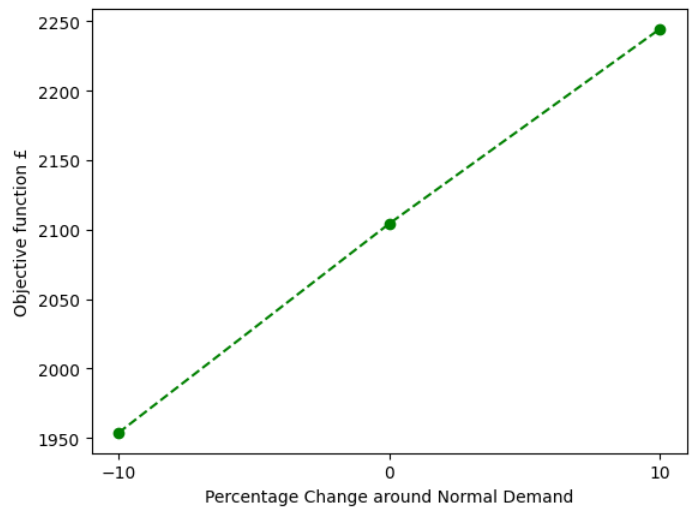
\includegraphics[scale=0.8]{Chapters/Chapter4New/Figures/WEDeterministicFinal.png}
    \caption{Objective Function Against Different Demand Levels - Deterministic Model}
    \label{fig:WEDeterministic}
\end{figure}

When comparing the low to average level demands, there is an increase of 10\% in the daily demands. In turn, this increases the total costs by \textcolor{blue}{7.70}\%. Similarly, the average to high level demand increase of 10\% shows there is an increase of 6.66\% in the objective function. The low to high daily demands cause an additional 20\% in demand, with a total increase of \textcolor{blue}{14.88}\% in costs.
% \begin{table}[h!]
%     \centering
%     \begin{tabular}{cccc} \toprule
%       \textbf{Decision Variable}  & \textbf{Low Level} & \textbf{Medium Level} & \textbf{High Level} \\\midrule
%         $x$^\textnormal{bed}_{1,1} & 91 & 87 &115 \\
%         $x$^\textnormal{bed}_{2,1} & 7 & 63 &8\\
%         $x$^\textnormal{bed}_{1,2} & 61 & 7& 135\\
%         $x$^\textnormal{bed}_{2,2} & 59 & 14&35\\
%         $x$^\textnormal{bed}_{1,3} & 14 & 103&75\\
%         $x$^\textnormal{bed}_{2,3} & 15 & 15&15\\ \midrule
%         $x$^\textnormal{staff}_{1,1,1} & 26.39 & 25.23 &35.35\\
%         $x$^\textnormal{staff}_{2,1,1} & 12.74 & 12.18 &16.1\\
%         $x$^\textnormal{staff}_{1,2,1} & 2.03 & 2.03&2.32\\
%         $x$^\textnormal{staff}_{2,2,1} & 1 & 1&1.12\\
%         $x$^\textnormal{staff}_{1,1,2} & 17.69 & 29.87&39.15\\
%         $x$^\textnormal{staff}_{2,1,2} & 8.54 & 14.42&18.9\\
%         $x$^\textnormal{staff}_{1,2,2} & 8.24 & 8.82&4.9\\
%         $x$^\textnormal{staff}_{2,2,2} & 17.11 & 18.27&10.15\\
%         $x$^\textnormal{staff}_{1,1,3} & 2 & 2&10.5\\
%         $x$^\textnormal{staff}_{2,1,3} & 4.06 & 4.06&21.75\\
%         $x$^\textnormal{staff}_{1,2,3} & 2.1 & 2.1 &2.1\\
%         $x$^\textnormal{staff}_{2,2,3} & 4.35 & 4.35&4.35\\\midrule
%          \textbf{Objective} &$\pounds$57,332.78 & $\pounds$67,028.28& $\pounds$90,962.98\\ \bottomrule
%     \end{tabular}
%     \caption{High, Medium, Low Level Demand Deterministic Results}
%     \label{tab:WEDeterministicResults}
% \end{table}

% When comparing the low to medium level demands, there is an increase in the 17.1024\% in the daily demand. In turn, this increases the total costs by 16.9101\%. Similarly, the medium to high level demand increase of 32.8184\% show there is an increase of 35.7084\%. The low to high daily demands cause an additional 58.6579\% in costs, with a 55.5336\% increase in demand.

% All three of these results show that increase in daily costs is directly proportional to the increase in daily demands.



\section{Two-Stage Stochastic Model Extension}\label{sec:twostagestochasticmodel}
The two-stage stochastic model is an extension of the deterministic model built in Section \ref{sec:DeterministicModel}. Since this is a two-stage model, Equations \eqref{eq:firststage} and \eqref{eq:secondstage} can be adapted in order to apply this to the case of bed and staffing capacity planning. \\\newline
All hospital beds are planned in advanced before the demand for each specialty and hospital is known. Similarly, nursing staff are deployed to specialties within the hospitals. When the demand is known, there is the option to change some specialty beds to alternative specialty beds with a cost. The two-stage version of this model enables various scenarios to be determined; if either the demand is changed, maximum capacities are changed or costs are changed. If the number of beds within the hospital is insufficient to satisfy the demand then a patient may be transferred to another hospital with availability or a new ward will open within the hospital, with a cost. The number of beds in total must not exceed the bed capacity for that hospital. Additionally, sufficient staff must be deployed to open beds, otherwise bank staff must be used.

The problem is to determine, for each hospital, the number of beds and staff required for each specialty in order to minimize the total costs, given by the sum of opening specialty beds within the hospital and the transportation costs of moving patients between hospitals. %The demand comes from the patient clusters identified in Section 3.1 and 3.2


\subsection{Sets}
In addition to the sets within the deterministic model, there are the set of scenarios in which different demands and situations can be run through the model.
\begin{table}[h!]
    \centering
    \begin{tabular}{ccl}\toprule
        \textbf{Parameter} & \textbf{Range} &\textbf{Definition} \\\midrule
       $\mathcal{B}$ & b = 1,..., B & \text{Set of nursing bands}\\
        $\mathcal{S}$ & s = 1,..., S & \text{Set of specialties} \\
    $\mathcal{H}$ & h = 1,..., H & \text{Set of hospitals} \\
    $\mathcal{R}$ & r = 1,..., R & \text{Set of regions}\\
    $\mathcal{K}$ & k = 1,..., K & \text{Set of scenarios}\\\bottomrule
    \end{tabular}
    \caption{Two-Stage Stochastic Model Sets}
    \label{tab:tssms}
\end{table}
% \begin{align*}
%     \mathcal{B} &= \{b:b=1,..., B\} : \text{set of nursing bands}\\
%     \mathcal{S} &= \{s:s = 1,..., S\} : \text{set of specialties} \\
%     \mathcal{H} &= \{h:h =1,..., H\} : \text{set of hospitals} \\
%     \mathcal{R} &= \{r:r=1,..., R\} : \text{set of regions}\\
%     \mathcal{K} &= \{k:k=1,..., K\} : \text{set of scenarios}\\
% \end{align*}

\subsection{Parameters}
\textcolor{blue}{Table \ref{tab:tssmp} denotes the parameters used within the two-stage stochastic model, along with a definition for each parameter.}
\begin{table}[h!]
    \centering
    \begin{tabular}{cl}\toprule
        \textbf{Parameter} & \textbf{Definition}  \\\midrule
            c^\textnormal{bed, 1st}_{s,h}& \text{Cost of the first stage beds for specialty $s\in\mathcal{S}$, in hospital $h\in\mathcal{H}$}\\ [0.2cm]
    c^\textnormal{bed, 2nd}_{s,h}& \text{Cost of the second stage beds for specialty $s\in\mathcal{S}$, in hospital $h\in\mathcal{H}$}\\ [0.2cm]
    c^\textnormal{staff, 1st}_{b}& \text{Cost of the first stage staff of band $b\in\mathcal{B}$}\\ [0.2cm]
    c^\textnormal{staff, 2nd}_{b}& \text{Cost of the second stage staff of band $b\in\mathcal{B}$}\\ [0.2cm]
    p_{k}&  \text{Probability of scenario $k \in \mathcal{K}$}\\ [0.2cm]
    P_{r,h}&  \text{Preference matrix of patients from region $r\in\mathcal{R}$ to hospital $h\in\mathcal{H}$}\\ [0.2cm]%This is given a cost factor
    D_{s,r,k} & \text{Demand for each speciality $s\in\mathcal{S}$, arriving from region $r\in\mathcal{R}$,} \\
   &\text{for scenario $k\in\mathcal{K}$}\\ [0.2cm]
    \textnormal{Min}^\textnormal{staff}_{s,h,k}& \text{Minimum number of staff required for specialty $s\in\mathcal{S}$, in hospital $h\in\mathcal{H}$,}\\
    &\text{for scenario $k\in\mathcal{K}$}\\ [0.2cm]
    R_{s,b} &\text{Ratio of nursing staff of band $b\in\mathcal{B}$ to patient for each specialty $s\in\mathcal{S}$}\\ [0.2cm]
    UB^\textnormal{max, bed, 1st}_{h} & \text{Upper bound of the number of beds that are able to be deployed }\\ 
    &\text{in hospital $h\in\mathcal{H}$ in the first stage}\\ [0.2cm]
    UB^\textnormal{max, bed, 2nd}_{h,k} & \text{Upper bound of the number of beds that are able to be deployed}\\
    &\text{in hospital $h\in\mathcal{H}$ in the second stage}\\ [0.2cm]
    UB^\textnormal{max, staff, 1st}_{b} & \text{Upper bound of the number of staff that can be deployed in the $1^{st}$ stage}\\[0.2cm]
    UB^\textnormal{max, staff, 2nd}_{b,k} & \text{Upper bound of the number of staff that can be deployed in the $2^{nd}$ stage} \\\bottomrule
    \end{tabular}
    \caption{Two-Stage Stochastic Model Parameters}
    \label{tab:tssmp}
\end{table}


% \begin{flushleft}
% \begin{align*}
%     c^\textnormal{bed, 1st}_{s,h}&: \text{Cost of the first stage beds for specialty $s\in\mathcal{S}$, in hospital $h\in\mathcal{H}$}\\
%     c^\textnormal{bed, 2nd}_{s,h}&: \text{Cost of the second stage beds for specialty $s\in\mathcal{S}$, in hospital $h\in\mathcal{H}$}\\
%     c^\textnormal{staff, 1st}_{b}&: \text{Cost of the first stage staff of band $b\in\mathcal{B}$}\\
%     c^\textnormal{staff, 2nd}_{b}&: \text{Cost of the second stage staff of band $b\in\mathcal{B}$}\\
%     p^{k}&: \text{Probability of scenario $k \in \mathcal{K}$}\\
%     P_{r,h} &: \text{Preference matrix of patients from region $r\in\mathcal{R}$ to hospital $h\in\mathcal{H}$}\\%This is given a cost factor
%     D_{s,r,k} &: \text{Demand for each speciality $s\in\mathcal{S}$ arriving from region $r\in\mathcal{R}$ } \\
%    &\phantom{:}\enspace\text{for each scenario $k\in\mathcal{K}$}\\
%     \textnormal{Min}^\textnormal{staff}_{s,h,k}&: \text{Minimum number of staff required for each specialty $s\in\mathcal{S}$}\\
%     &\phantom{:}\enspace\text{in each hospital $h\in\mathcal{H}$ for each scenario $k\in\mathcal{K}$}\\
%     R_{s,b} &:\text{Ratio of nursing staff of band $b\in\mathcal{B}$ to patient for each specialty $s\in\mathcal{S}$}\\
%     UB^\textnormal{max, bed, 1st}_{h} &: \text{Upper bound of the number of beds that are able to be deployed }\\
%     &\phantom{:}\enspace\text{in hospital $h\in\mathcal{H}$ in the first stage}\\
%     UB^\textnormal{max, bed, 2nd}_{h,k} &: \text{Upper bound of the number of beds that are able to be deployed}\\
%     &\phantom{:}\enspace\text{in hospital $h\in\mathcal{H}$ in the second stage}\\
%     UB^\textnormal{max, staff, 1st}_{b} &: \text{Upper bound of the number of staff that can be deployed in the $1^{st}$ stage}\\
%     UB^\textnormal{max, staff, 2nd}_{b,k} &: \text{Upper bound of the number of staff that can be deployed in the $2^{nd}$ stage}
% \end{align*}
% \end{flushleft}
\subsection{Decision Variables}
The decision variables \textcolor{blue}{that were listed in Table \ref{tab:dmdv} can be extended to include the second stage decision variables, given in Table \ref{tab:tssmdv}}.

\begin{table}[h!]
    \centering
    \begin{tabular}{cl}\toprule
        \textbf{Decision Variable} & \textbf{Definition} \\\midrule
         $x^\textnormal{bed}_{s,h}$ \in \mathbb{N} & \text{Number of beds planned in the $1^{st}$ stage for specialty $s\in\mathcal{S}$,} \\
         & {in hospital $h\in\mathcal{H}$} \\ [0.2cm]

     $x^\textnormal{staff}_{s,b,h}$ \in \mathbb{R} &\text{Number of staff planned in the $1^{st}$ stage for specialty $s\in\mathcal{S}$,} \\
    & {of band $b\in\mathcal{B}$, in hospital $h\in\mathcal{H}$}\\ [0.2cm]
    $u^\textnormal{bed}_{s,r,h,k} $ \in \mathbb{N} &\text{Number of beds needed in the $2^{nd}$ stage for specialty $s\in\mathcal{S}$,}\\
   & {for patients arriving from region $r\in\mathcal{R}$ in hospital $h\in\mathcal{H}$,}\\
   & {for scenario $k\in\mathcal{K}$} \\   [0.2cm]
   $ u^\textnormal{staff}_{s,b,h,k}$ \in \mathbb{R} & \text{Number of staff needed in the $2^{nd}$ stage for specialty $s\in\mathcal{S}$,} \\
   &{of band $b\in\mathcal{B}$, in hospital $h\in\mathcal{H}$, for scenario $k\in\mathcal{K}$} \\  \bottomrule 
    \end{tabular}
    \caption{Two-Stage Stochastic Model Decision Variables}
    \label{tab:tssmdv}
\end{table}

% \begin{align*}
%    x^\textnormal{bed}_{s,h} \in \mathbb{N} &: \text{Number of beds planned in the $1^{st}$ stage for specialty $s\in\mathcal{S}$} \\
%    &\phantom{:}\enspace \text{in hospital $h\in\mathcal{H}$}\\
%     x^\textnormal{staff}_{s,b,h} \in \mathbb{R} &:\text{number of staff planned in the $1^{st}$ stage for specialty $s\in\mathcal{S}$ }\\
%     &\phantom{:}\enspace \text{of band $b\in\mathcal{B}$ in hospital $h\in\mathcal{H}$}\\
%    u^\textnormal{bed}_{s,r,h,k} \in \mathbb{N} &:\text{number of beds needed in the $2^{nd}$ stage for specialty $s\in\mathcal{S}$ for patients } \\
%    &\phantom{:}\enspace \text{arriving from region $r\in\mathcal{R}$ in hospital $h\in\mathcal{H}$ for scenario $k\in\mathcal{K}$} \\  
%    u^\textnormal{staff}_{s,b,h,k} \in \mathbb{R} &: \text{number of staff needed in the $2^{nd}$ stage for specialty $s\in\mathcal{S}$ } \\
%    &\phantom{:}\enspace \text{of band $b\in\mathcal{B}$ in hospital $h\in\mathcal{H}$ for scenario $k\in\mathcal{K}$} \\  
% \end{align*}

\subsection{Model}
The following two-stage stochastic model can be determined, adapted from Equations \eqref{eq:det_objective} - \eqref{eq:det_con5}, resulting in the Equations \eqref{eq:sto_objective} - \eqref{eq:sto_con7}.

\begin{multline}\label{eq:sto_objective}
    \text{min} \sum_{h\in\mathcal{H}}\sum_{s\in\mathcal{S}}(x^\textnormal{bed}_{s,h}c^\textnormal{bed, 1st}_{s,h} + \sum_{b\in\mathcal{B}}x^\textnormal{staff}_{s,b,h}c^\textnormal{staff, 1st}_{b}) +\\ 
    \sum_{k\in\mathcal{K}}\sum_{h\in\mathcal{H}}\sum_{s\in\mathcal{S}}p_{k}(\sum_{r\in\mathcal{R}} P_{r,h} u^\textnormal{bed}_{s,r,h,k}c^\textnormal{bed, 2nd}_{s,h} +
   \sum_{b\in\mathcal{B}} u^\textnormal{staff}_{s,b,k,h}c^\textnormal{staff, 2nd}_{b})
\end{multline}


subject to:
\begin{align}
    \sum_{h\in\mathcal{H}} x^\textnormal{bed}_{s,h} +  \sum_{h\in\mathcal{H}} u^\textnormal{bed}_{s,r,h,k} \geq D_{s,r,k} & & \forall r \in \mathcal{R}, s \in \mathcal{S}, k \in \mathcal{K} \label{eq:sto_con1}\\
    \sum\limits_{b\in\mathcal{B}} \left(x^\textnormal{staff}_{s,b,h} +u^\textnormal{staff}_{s,b,k,h} \right) \geq \textnormal{Min}^\textnormal{staff}_{s,h,k}& & \forall s \in \mathcal{S}, k \in \mathcal{K}, h \in \mathcal{H} \label{eq:sto_con2}\\ 
    \sum\limits_{b'\in\mathcal{B}: b'\geq b} x^\textnormal{staff}_{s,b',h} + u^\textnormal{staff}_{s,b',k,h} \geq R_{s,b} \cdot (x^\textnormal{bed}_{s,h} +  \sum\limits_{r\in\mathcal{R}} u^\textnormal{bed}_{s,r,h,k} ) & & \forall b \in \mathcal{B}, s \in \mathcal{S}, k \in \mathcal{K}, h \in \mathcal{H}\label{eq:sto_con3}\\
    0 \leq x^\textnormal{bed}_{s,h} \leq UB^\textnormal{max, bed, 1st}_h & &\forall s \in \mathcal{S}, h \in \mathcal{H}\label{eq:sto_con4}\\
    0 \leq x^\textnormal{staff}_{s,b,h} \leq UB^\textnormal{max, staff, 1st}_{b}& & \forall s \in \mathcal{S}, b \in \mathcal{B}, h \in \mathcal{H}\label{eq:sto_con5}\\
    0 \leq u^\textnormal{bed}_{s,h,k} \leq UB_h^\textnormal{max, bed, 2nd} & & \forall s \in \mathcal{S}, k \in \mathcal{K},  h \in \mathcal{H}\label{eq:sto_con6}\\
    0 \leq u^\textnormal{staff}_{s,b,k,h} \leq UB^\textnormal{max, staff, 2nd}_{b}& & \forall s \in \mathcal{S}, b \in \mathcal{B}, k \in \mathcal{K}, h \in \mathcal{H}\label{eq:sto_con7}
\end{align}

The first sum in the objective function \eqref{eq:sto_objective} is the cost of deploying both beds and staff to specialties within each hospital. The second sum represents the additional beds and staff within the same hospital or a different hospital in the region. The first constraint, \eqref{eq:sto_con1}, assures the demand for each specialty and region is met by the number of hospital beds deployed. Constraint \eqref{eq:sto_con2} ensures the number of staff deployed meets the minimum requirements for staff on each specialty ward. The final constraint \eqref{eq:sto_con3} ensures the staff to bed ratio is met. Equations \eqref{eq:sto_con4} - \eqref{eq:sto_con7} define the maximum bounds on the first and second stage decision variables of the problem.\\

\subsection{Worked Example}

Using the fifteen patients discussed previously, these can be applied to the two-stage stochastic model. Table \ref{tab:DeterministicWorkedExample} can be extended to include the second stage model.


\begin{table}[h!]
    \centering
    \begin{tabular}{ll}\toprule
       \textbf{Parameters}  & \textbf{Values} \\\midrule
        1$^{st}$ Stage Bed Costs ($c^\textnormal{bed,1st}_{s,h}$) & $\begin{bmatrix} 20 & 30 \\ 30 & 40 \end{bmatrix}$\\  [0.5cm]
        2$^{st}$ Stage Bed Costs ($c^\textnormal{bed,2nd}_{s,h}$) & $\begin{bmatrix} 22 & 33 \\ 33 & 44 \end{bmatrix}$\\ [0.5cm]
        Ratio ($R_{s,b}$) &$\begin{bmatrix}0.29&0.14\\
         0.14&0.29\end{bmatrix}$\\ [0.5cm]
         Minimum Staffing Levels ($\textnormal{Min}^\textnormal{staff}_{s,h,k}$) &$\begin{bmatrix}
         [1,1]&[2,2]  \\
         [1,1]&[3,3]\\
         \end{bmatrix}$\\[0.5cm]
         1$^{st}$ Stage Staff Costs ($c^\textnormal{staff, 1st}_{b}$) &[$\pounds50, \pounds60$] \\ [0.25cm]
         2$^{nd}$ Stage Staff Costs ($c^\textnormal{staff, 2nd}_{b}$) &[$\pounds55, \pounds66$] \\ [0.25cm]
         Upper 1$^{st}$ bed limit ($UB^\textnormal{max,bed,1st}_{h}$) &  [20,25]\\[0.25cm]
         Upper 2$^{nd}$ bed limit ($UB^\textnormal{max,bed,2nd}_{h,k}$) &  $\begin{bmatrix} 20 & 20 &20\\ 25 & 25 &25 \end{bmatrix}$\\[0.5cm]
         Upper 1$^{st}$ staff limit ($UB^\textnormal{max,staff,1st}_{b}$)& [15,25]\\[0.25cm]
         Upper 2$^{nd}$ staff limit ($UB^\textnormal{max,staff,2nd}_{b.k}$)& $\begin{bmatrix} 15 & 15 \\ 25 & 25 \end{bmatrix}$\\[0.5cm]
         Preference Matrix ($P_{r,h}$) & [1,1]\\[0.25cm]
         Probability of Scenarios ($p_{k}$) & [0.4,0.3,0.3]\\
         
         \bottomrule
    \end{tabular}
    \caption{Deterministic Parameter Values for the Worked Example}
    \label{tab:DeterministicWorkedExample}
\end{table}

\textcolor{blue}{The matrices are stored in row-major order. For the terms with three indices, e.g., $\textnormal{Min}^{\textnormal{staff}}_{s,h,k}$, the first index refers to row and the second index corresponds to the column. The third index refers to column inside the sub-matrix. To illustrate, if we refer to the first hospital and specialty ($\textnormal{Min}^{\textnormal{staff}}_{1,1,k}$), then, if $k=1$, we refer to the first element inside the [1,1] matrix. If $k=2$, we refer to the second element inside the [1,1]. In each instance this value is one.}

Similarly, Equations \eqref{eq:averagebeds1} and \eqref{eq:averagebeds2} can be used to determine the average daily bed demand. Three scenarios for the more are studied:

\begin{itemize}
    \item Average demand with a probability of 40\%
    \item Demand increasing by 20\% with a probability of 30\% 
    \item Demand decrease by 20\% with a probability of 30\%
\end{itemize}

The model is additionally run with the low demand (-10\%) and high demand (+10\%) with the same scenario percentages.
\begin{table}[h!]
    \centering
    \begin{tabular}{cccccccccc}\toprule
    \textbf{} & \multicolumn{3}{c}{\textbf{Low Demand}}
         &  \multicolumn{3}{c}{\textbf{Average Demand}} & \multicolumn{3}{c}{\textbf{High Demand}}\\
         & \textbf{k=1} & \textbf{k=2} & \textbf{k=3}& \textbf{k=1} & \textbf{k=2} & \textbf{k=3} & \textbf{k=1} & \textbf{k=2} & \textbf{k=3} \\
         \midrule
        $D_{0,0,k}$ & 15.001 & 18.002 & 12.001 & 16.66 & 19.992 & 13.328 & 18.33 & 21.996 & 14.664 \\
        $D_{0,0,k}$ & 17.10  & 20.52  & 13.68  & 19.0  & 22.8   & 15.2   & 20.9  & 25.08  & 16.72 \\ \bottomrule
    \end{tabular}
    \caption{Demands for the Two-Stage Stochastic Model and Scenarios}
    \label{tab:WEStochDemands}
\end{table}


Table \ref{tab:WEStochDemands} displays the demands for each scenario of the low, average and high demands for the two-stage stochastic problem. 



These demands can be input into the two-stage stochastic model to obtain the objective function for each case. Table \ref{tab:WEStochResults} shows the values for each of the decision variables, $x^{\textnormal{bed}}_{s,h}$, $x^{\textnormal{staff}}_{s,b,h}$, $x^{\textnormal{bed}}_{s,r,h,k}$ and $u^{\textnormal{staff}}_{s,b,h,k}$, is displayed.

\begin{landscape}
\begin{table}[h!]
    \centering
    \begin{tabular}{cccccccccc}\toprule
\textbf{$1^{st}$ Stage Decision Variables} & \multicolumn{3}{c}{\textbf{Low Demand}} & \multicolumn{3}{c}{\textbf{Average Demand}} & \multicolumn{3}{c}{\textbf{High Demand}} \\\midrule

    $x^\textnormal{bed}_{0,0}$        &\multicolumn{3}{c}{4}  &\multicolumn{3}{c}{4}    &\multicolumn{3}{c}{4}    \\
    $x^\textnormal{bed}_{0,1}$        &\multicolumn{3}{c}{6}  &\multicolumn{3}{c}{7}    &\multicolumn{3}{c}{7}    \\
    $x^\textnormal{bed}_{1,0}$        &\multicolumn{3}{c}{4}  &\multicolumn{3}{c}{4}    &\multicolumn{3}{c}{4}    \\
    $x^\textnormal{bed}_{1,1}$        &\multicolumn{3}{c}{10} &\multicolumn{3}{c}{10}   &\multicolumn{3}{c}{10}   \\ \midrule
    $x^\textnormal{staff}_{0,0,0}$    &\multicolumn{3}{c}{1.16} &\multicolumn{3}{c}{1.16} &\multicolumn{3}{c}{1.16} \\
    $x^\textnormal{staff}_{0,0,1}$    &\multicolumn{3}{c}{1.0}  &\multicolumn{3}{c}{1.0}  &\multicolumn{3}{c}{1.0}  \\
    $x^\textnormal{staff}_{0,1,0}$    &\multicolumn{3}{c}{2.0}  &\multicolumn{3}{c}{2.03} &\multicolumn{3}{c}{2.03} \\
    $x^\textnormal{staff}_{0,1,1}$    &\multicolumn{3}{c}{2.0}  &\multicolumn{3}{c}{2.0}  &\multicolumn{3}{c}{2.0}  \\
    $x^\textnormal{staff}_{1,0,0}$    &\multicolumn{3}{c}{1.0}  &\multicolumn{3}{c}{1.0}  &\multicolumn{3}{c}{1.0}  \\
    $x^\textnormal{staff}_{1,0,1}$    &\multicolumn{3}{c}{1.16} &\multicolumn{3}{c}{1.16} & \multicolumn{3}{c}{1.16}\\
    $x^\textnormal{staff}_{1,1,0}$    &\multicolumn{3}{c}{3.0}  &\multicolumn{3}{c}{3.0}  &\multicolumn{3}{c}{3.0}  \\
    $x^\textnormal{staff}_{1,1,1}$    &\multicolumn{3}{c}{3.0}  &\multicolumn{3}{c}{3.0}  & \multicolumn{3}{c}{3.0} \\ \midrule
     \textbf{$2^{nd}$ Stage Decision Variables} & \multicolumn{3}{c}{\textbf{Low Demand}} & \multicolumn{3}{c}{\textbf{Average Demand}} & \multicolumn{3}{c}{\textbf{High Demand}} \\
     & \textbf{k=1} & \textbf{k=2} & \textbf{k=3}& \textbf{k=1} & \textbf{k=2} & \textbf{k=3}& \textbf{k=1} & \textbf{k=2} & \textbf{k=3}\\
     \midrule
    $u^\textnormal{bed}_{0,0,k}$     & 4  & 4  & 3  & 4  & 4  & 3  & 4  & 4  & 4  \\
    $u^\textnormal{bed}_{0,1,k}$     & 2  & 5  & 0  & 2  & 5  & 0  & 4  & 7  & 0  \\
    $u^\textnormal{bed}_{1,0,k}$     & 4  & 4  & 0  & 4  & 4  & 2  & 4  & 4  & 3  \\
    $u^\textnormal{bed}_{1,1,k}$     & 0  & 3  & 0  & 1  & 5  & 0  & 3  & 8  & 0  \\ \midrule
    $u^\textnormal{staff}_{0,0,0,k}$ & 1.16 & 1.16 & 1.0  & 1.16 & 1.16 & 1.0  & 1.16 & 1.16 & 1.16 \\
    $u^\textnormal{staff}_{0,0,1,k}$ & 1.0  & 1.0  & 1.0  & 1.0  & 1.0  & 1.0  & 1.0  & 1.0  & 1.0  \\
    $u^\textnormal{staff}_{0,1,0,k}$ & 2.0  & 2.0  & 2.0  & 2.0  & 2.0  & 2.0  & 2.0  & 2.03 & 2.0  \\
    $u^\textnormal{staff}_{0,1,1,k}$ & 2.0  & 2.0  & 2.0  & 2.0  & 2.0  & 2.0  & 2.0  & 2.0  & 2.0  \\
    $u^\textnormal{staff}_{1,0,0,k}$ & 1.0  & 1.0  & 1.0  & 1.0  & 1.0  & 1.0  & 1.0  & 1.0  & 1.0  \\
    $u^\textnormal{staff}_{1,0,1,k}$ & 1.16 & 1.16 & 1.0  & 1.16 & 1.16 & 1.0  & 1.16 & 1.16 & 1.0  \\
    $u^\textnormal{staff}_{1,1,0,k}$ & 3.0  & 3.0  & 3.0  & 3.0  & 3.0  & 3.0  & 3.0  & 3.0  & 3.0  \\
    $x^\textnormal{staff}_{1,1,1,k}$ & 3.0  & 3.0  & 3.0  & 3.0  & 3.0  & 3.0  & 3.0  & 3.0  & 3.0  \\ \midrule
     \textbf{\textcolor{blue}{Objective Function Value}} &\multicolumn{3}{c}{$\pounds$2,717.45} & \multicolumn{3}{c}{$\pounds$2,812.75}& \multicolumn{3}{c}{$\pounds$2,953.39 }\\\bottomrule
    \end{tabular}
    \caption{High, Average and Low Level Demand Two-Stage Stochastic Results}
    \label{tab:WEStochResults}
\end{table}

\end{landscape}

The RP values for the three demand levels are $\pounds$2,717.45, $\pounds$2,812.75, $\pounds$2,953.39 for the low, average and high levels of demands. 

\begin{figure}[h!]
    \centering
    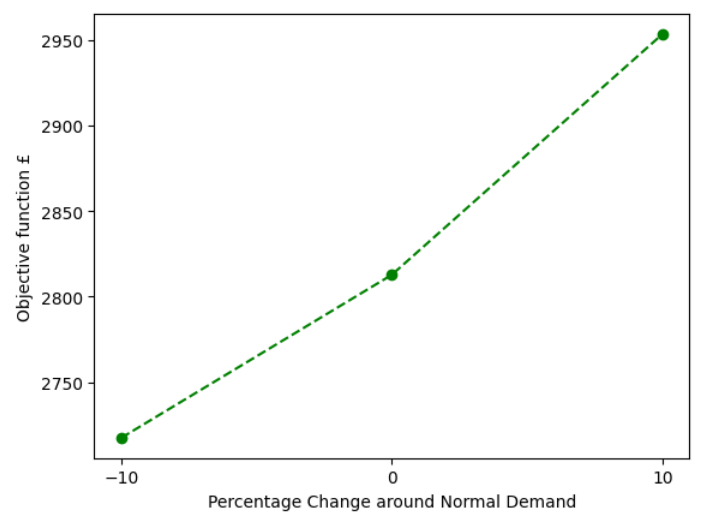
\includegraphics[scale=0.75]{Chapters/Chapter4New/Figures/WEStochastic.png}
    \caption{Objective Function Against Different Demand Levels - Two-Stage Stochastic Model}
    \label{fig:WEStochastic}
\end{figure}

The low to average level demands show only a 3.51\% increase despite a 10\% increase in demand. Similarly, average to high level demands yield a 5\% increase. The low to high daily demands cause an additional 20\% in costs, with a total increase of 8.68\% in demands.

These three cases have only a small increase due to constraint \eqref{eq:sto_con2}, where the minimum level of staff must be met. In this case, due to the small number of beds allocated, staff are being assigned to wards where there are either no beds, or such quantity of staff is much higher than the original ratio.


\section{Evaluation of Measures}\label{sec:evalofmeasures}
This section looks at applying the three tests discussed in Sections \ref{sec:TestA}, \ref{sec:TestB} and \ref{sec:TestC} to the worked example of frail and elderly patient services. Furthermore, it will determine how the results can be evaluated and determine where the model is under performing.


\subsection{Test A}
Test A involves calculating the VSS to determine the expected loss when using the deterministic solution. If we recall Equations \eqref{eq:EEV} and \eqref{eq:VSS}, which calculates the EEV and VSS respectively.

\begin{equation}
    EEV = E_{\boldsymbol{\xi}} (z(\bar x (\bar \xi),\boldsymbol{\xi})) \tag{\ref{eq:EEV} revisited}
\end{equation}
\begin{equation}
    VSS = EEV - RP\tag{\ref{eq:VSS} revisited}
\end{equation}

Tables \ref{tab:WELowDemandTestA} - \ref{tab:WEHighDemandTestA} display the results for calculating the VSS for the worked example, with low, average and high demand respectively. The deterministic model deploys fewer beds and nursing staff than the stochastic model in each of the three cases, leading to an EV solution that costs around only two-thirds of the RP. However, the EEV is larger in all cases and this results in the following VSS scores:
\begin{align}
    VSS_{Low} &= 2881.70 - 2717.45 = 164.25 (1\%)\\
    VSS_{Average} &= 3031.20 - 2812.75 = 218.45 (7\%)\\
    VSS_{High} &= 3120.61 - 2935.39 = 185.22 (5\%)
\end{align}

This demonstrates that utilising the stochastic model rather than the deterministic, can save \textcolor{blue}{between 1\% and 7\% in bed and staffing costs.}
\begin{table}[h!]
    \centering\scalebox{0.75}{
    \begin{tabular}{l|cccc|l} \toprule
         & \textbf{s=0, h=0} & \textbf{s=0, h=1}  &\textbf{s=1, h=0}  &\textbf{s=1, h=1}  & \textbf{Objective Value ($\pounds$)}\\ \midrule
        Deterministic & [(7), (2.01, 1)] & [(9), (2, 2)] & [(7), (1, 2.03)] & [(11), (3, 3.19)] & 1935.70 = EV\\
        Stochastic & [(8), (2.32, 2)] & [(11), (4, 4)] & [(8), (2, 2.32)] &[(13), (6, 6)] & 2717.45 = RP\\
        Test A  & [(10), (3.03, 2)] & [(9), (4.61,4)] & [(10), (2,3.03)] & [(14), (6,6.19)] & 2881.70 = EEV\\\bottomrule
    \end{tabular}}
    \caption{Low Demand Worked Example where results are recorded [(beds), (staff)] - Test A Results}
    \label{tab:WELowDemandTestA}
\end{table}

\begin{table}[h!]
    \centering\scalebox{0.75}{
    \begin{tabular}{l|cccc|l} \toprule
         & \textbf{s=0, h=0} & \textbf{s=0, h=1}  &\textbf{s=1, h=0}  &\textbf{s=1, h=1}  & \textbf{Objective Value ($\pounds$)}\\ \midrule
        Deterministic & [(8), (2.32,1.12)] & [(9), (2, 2)] & [(9), (1.26, 2.61)] & [(11), (3, 3)] & 2104.20= EV\\
        Stochastic & [(8), (2.32, 2)] & [(12), (4.03, 4)] & [(8), (2, 2.32)] &[(15), (6, 6)] &  2812.75= RP\\
        Test A  & [(11), (3.32, 2.12)] & [(9), (4.61, 4)] & [(12), (2.26, 3.61)] & [(11), (6, 6.19)] & 3031.20 = EEV\\\bottomrule
    \end{tabular}}
    \caption{Average Demand Worked Example where results are recorded [(beds), (staff)] - Test A Results}
    \label{tab:WENorDemandTestA}
\end{table}
\begin{table}[h!]
    \centering\scalebox{0.75}{
    \begin{tabular}{l|cccc|l} \toprule
         & \textbf{s=0, h=0} & \textbf{s=0, h=1}  &\textbf{s=1, h=0}  &\textbf{s=1, h=1}  & \textbf{Objective Value ($\pounds$)}\\ \midrule
        Deterministic & [(10), (2.9, 1.4)] & [(9), (2, 2)] & [(10), (1.4, 2.9)] & [(11), (3, 3.19)] & 2244.40 = EV\\
        Stochastic & [(8, (2.32, 2)] & [(14), (4.06, 4)] & [(8), (2, 2.32)] &[(18), (6, 6)] & 2953.39 = RP\\
        Test A  & [(12), (3.48, 2.12)] & [(10), (4.61, 4)] & [(13), (2.26, 3.77)] & [(13), (6, 6.19)] & 3120.61 = EEV\\\bottomrule
    \end{tabular}}
    \caption{High Demand Worked Example where results are recorded [(beds), (staff)] - Test A Results}
    \label{tab:WEHighDemandTestA}
\end{table}

% $x^{\textnormal{bed}}_{s,h}$, $x^{\textnormal{staff}}_{s,b,h}$,
% can be applied to the case of frail and elderly patients.
% In order for the VSS to be calculated, the EEV requires to be calculated. 

To determine the exact reason as to why the deterministic model performed poorly, further tests can be performed.

\subsection{Test B}
Test B takes the skeleton solution from the deterministic model. Since the deterministic model did not result in any zero values being produced, the lower bound values instead will be taken. 

We calculate the ESSV as follows:
\begin{equation}
    ESSV = E_{\boldsymbol{\xi}}(z(\hat x, \boldsymbol{\xi})) \tag{\ref{eq:ESSV} revisited} 
\end{equation}
and then use this information to calculate the LUSS:
\begin{equation}
    LUSS = ESSV - RP\tag{\ref{eq:LUSS} revisited}
\end{equation}

Tables \ref{tab:WELowDemandTestB} - \ref{tab:WEHighDemandTestB}, present the results after the ESSV calculations have been calculated. For each case, the ESSV is larger than the RP and therefore the LUSS is as follows:
\vspace{-0.25cm}
\begin{align}
    LUSS_{Low} & = 2753.15 - 2717.45 = 35.7\\
    LUSS_{Average} & = 2836.45 - 2812.75 = 23.7\\
    LUSS_{High} & = 2979.85 - 2953.39  = 26.46
\end{align}

Since the model is fixed by how many beds it can deploy in the first stage, the demand is not satisfied within the first stage. The model reacts by opening beds in the second stage, in the facilities where this is restricted in the first stage. This occurs because the second stage costs for some bed specialties is in fact less expensive than first stage costs in other bed specialties.


\begin{table}[h!]
    \centering\scalebox{0.75}{
    \begin{tabular}{l|cccc|l} \toprule
         & \textbf{s=0, h=0} & \textbf{s=0, h=1}  &\textbf{s=1, h=0}  &\textbf{s=1, h=1}  & \textbf{Objective Value ($\pounds$)}\\ \midrule
        Deterministic & [(7), (2.01, 1)] & [(9), (2, 2)] & [(7), (1, 2.03)] & [(11), (3, 3.19)] & 1935.70 = EV\\
        Stochastic & [(8), (2.32, 2)] & [(11), (4, 4)] & [(8), (2, 2.32)] &[(13), (6, 6)] & 2717.45 = RP\\
        Test A  & [(10), (3.03, 2)] & [(9), (4.61,4)] & [(10), (2,3.03)] & [(14), (6,6.19)] & 2881.70 = EEV\\
        Test B & [(11) , (3.19, 2)] & [(8) , (4, 4)] & [(11) , (2, 3.19)] & [(10) , (6, 6)] &2753.15 = ESSV \\\bottomrule
    \end{tabular}}
    \caption{Low Demand Worked Example where results are recorded [(beds), (staff)] - Test B Results}
    \label{tab:WELowDemandTestB}
\end{table}

\begin{table}[h!]
    \centering\scalebox{0.75}{
    \begin{tabular}{l|cccc|l} \toprule
         & \textbf{s=0, h=0} & \textbf{s=0, h=1}  &\textbf{s=1, h=0}  &\textbf{s=1, h=1}  & \textbf{Objective Value ($\pounds$)}\\ \midrule
        Deterministic & [(8), (2.32,1.12)] & [(9), (2, 2)] & [(9), (1.26, 2.61)] & [(11), (3, 3)] & 2104.20= EV\\
        Stochastic & [(8), (2.32, 2)] & [(12), (4.03, 4)] & [(8), (2, 2.32)] &[(15), (6, 6)] &  2812.75= RP\\
        Test A  & [(11), (3.32, 2.12)] & [(9), (4.61, 4)] & [(12), (2.26, 3.61)] & [(11), (6, 6.19)] & 3031.20 = EEV\\
        Test B & [(12), (3.48, 2.12)] & [(8), (4, 4)] & [(8), (2, 2.32)]  & [(15), (6, 6)]  & 2836.45 = ESSV\\ \bottomrule
    \end{tabular}}
    \caption{Average Demand Worked Example where results are recorded [(beds), (staff)] - Test B Results}
    \label{tab:WENorDemandTestB}
\end{table}
\begin{table}[h!]
    \centering\scalebox{0.75}{
    \begin{tabular}{l|cccc|l} \toprule
         & \textbf{s=0, h=0} & \textbf{s=0, h=1}  &\textbf{s=1, h=0}  &\textbf{s=1, h=1}  & \textbf{Objective Value ($\pounds$)}\\ \midrule
        Deterministic & [(10), (2.9, 1.4)] & [(9), (2, 2)] & [(10), (1.4, 2.9)] & [(11), (3, 3.19)] & 2244.40 = EV\\
        Stochastic & [(8, (2.32, 2)] & [(14), (4.06, 4)] & [(8), (2, 2.32)] &[(18), (6, 6)] & 2953.39 = RP\\
        Test A  & [(12), (3.48, 2.12)] & [(10), (4.61, 4)] & [(13), (2.26, 3.77)] & [(13), (6, 6.19)] & 3120.61 = EEV\\
        Test B & [(8), (2.32, 2)] & [(14), (4.61, 4)]  & [(8), (2, 2.32)]  & [(18), (6, 6)] & 2979.85= ESSV \\\bottomrule
    \end{tabular}}
    \caption{High Demand Worked Example where results are recorded [(beds), (staff)] - Test B Results}
    \label{tab:WEHighDemandTestB}
\end{table}


\subsection{Test C}
Test C determines the upgradeability of the model. The number of beds and staff deployed in the deterministic solution are added as constraints, where these minimum numbers have to be met in the first stage. Equation \ref{eq:EIV} calculates the expectant result from this test:

\begin{equation}
    EIV = E_{\boldsymbol{\xi}}(z(\Tilde{x},\boldsymbol{\xi})) \tag{\ref{eq:EIV} revisited}
\end{equation}
\begin{equation}
    LUDS = EIV - RP \tag{\ref{eq:LUDS} revisited}
\end{equation}
The LUDS values for each case are as follows:
\begin{align}
    LUDS_{Low} &= 2881.70 - 2881.70 = 0 \\
    LUDS_{Average} &= 3031.20 - 3031.20 = 0 \\
    LUDS_{High} &= 3197.67 - 3120.61 = 77.06
\end{align}
Tables \ref{tab:WELowDemandTestC} - \ref{tab:WEHighDemandTestC} display the results for the EIV. For the low and average level demands, the results show that the EIV is equal to RP, showing perfect upgradeability of the deterministic solution. For the high level of demand case, the LUDS value is less than the VSS (0 $<$ 77.06 (LUDS) $<$ 185.22 (VSS)), and therefore there is partial upgradeability.




\begin{table}[h!]
    \centering\scalebox{0.75}{
    \begin{tabular}{l|cccc|l} \toprule
         & \textbf{s=0, h=0} & \textbf{s=0, h=1}  &\textbf{s=1, h=0}  &\textbf{s=1, h=1}  & \textbf{Objective Value ($\pounds$)}\\ \midrule
        Deterministic & [(7), (2.01, 1)] & [(9), (2, 2)] & [(7), (1, 2.03)] & [(11), (3, 3.19)] & 1935.70 = EV\\
        Stochastic & [(8), (2.32, 2)] & [(11), (4, 4)] & [(8), (2, 2.32)] &[(13), (6, 6)] & 2717.45 = RP\\
        Test A  & [(10), (3.03, 2)] & [(9), (4.61,4)] & [(10), (2,3.03)] & [(14), (6,6.19)] & 2881.70 = EEV\\
        Test B & [(11), (3.19, 2)] & [(8), (4, 4)] & [(11), (2, 3.19)] & [(10), (6, 6)] &2753.15 = ESSV \\
        Test C  & [(10), (3.03, 2)] & [(9), (4.61,4)] & [(10), (2,3.03)] & [(14), (6,6.19)] & 2881.70 = EIV = EEV \\\bottomrule
    \end{tabular}}
    \caption{Low Demand Worked Example where results are recorded [(beds), (staff)] - Test C Results}
    \label{tab:WELowDemandTestC}
\end{table}

\begin{table}[h!]
    \centering\scalebox{0.72}{
    \begin{tabular}{l|cccc|l} \toprule
         & \textbf{s=0, h=0} & \textbf{s=0, h=1}  &\textbf{s=1, h=0}  &\textbf{s=1, h=1}  & \textbf{Objective Value ($\pounds$)}\\ \midrule
        Deterministic & [(8), (2.32,1.12)] & [(9), (2, 2)] & [(9), (1.26, 2.61)] & [(11), (3, 3)] & 2104.20= EV\\
        Stochastic & [(8), (2.32, 2)] & [(12), (4.03, 4)] & [(8), (2, 2.32)] &[(15), (6, 6)] &  2812.75= RP\\
        Test A  & [(11), (3.32, 2.12)] & [(9), (4.61, 4)] & [(12), (2.26, 3.61)] & [(11), (6, 6.19)] & 3031.20 = EEV\\
        Test B & [(12), (3.48, 2.12)] & [(8), (4, 4)] & [(8), (2, 2.32)]  & [(15), (6, 6)]  & 2836.45 = ESSV\\ 
        Test C  & [(11), (3.32, 2.12)] & [(9), (4.61, 4)] & [(12), (2.26, 3.61)] & [(11), (6, 6.19)] & 3031.20 = EIV = EEV\\\bottomrule
    \end{tabular}}
    \caption{Average Demand Worked Example where results are recorded [(beds), (staff)] - Test C Results}
    \label{tab:WENorDemandTestC}
\end{table}
\begin{table}[h!]
    \centering\scalebox{0.72}{
    \begin{tabular}{l|cccc|l} \toprule
         & \textbf{s=0, h=0} & \textbf{s=0, h=1}  &\textbf{s=1, h=0}  &\textbf{s=1, h=1}  & \textbf{Objective Value ($\pounds$)}\\ \midrule
        Deterministic & [(10), (2.9, 1.4)] & [(9), (2, 2)] & [(10), (1.4, 2.9)] & [(11), (3, 3.19)] & 2244.40 = EV\\
        Stochastic & [(8, (2.32, 2)] & [(14), (4.06, 4)] & [(8), (2, 2.32)] &[(18), (6, 6)] & 2953.39 = RP\\
        Test A  & [(12), (3.48, 2.12)] & [(10), (4.61, 4)] & [(13), (2.26, 3.77)] & [(13), (6, 6.19)] & 3120.61 = EEV\\
        Test B & [(8), (2.32, 2)] & [(14), (4.61, 4)]  & [(8), (2, 2.32)]  & [(18), (6, 6)] & 2979.85= ESSV \\
        Test C & [(13), (3.9, 2.4)] & [(9), (4.61, 4)] & [(14), (2.4, 4.06)] &[(12), (6, 6.19)] & 3197.67 = EIV\\\bottomrule
    \end{tabular}}
    \caption{High Demand Worked Example where results are recorded [(beds), (staff)] - Test C Results}
    \label{tab:WEHighDemandTestC}
\end{table}

\subsection{Worked Example Conclusion}
The worked example provided three low, average and high demand scenarios to determine how beds and staff can be planned for two specialities within two hospitals. These cases were performed in both a deterministic and stochastic environment, to replicate both real world planning and real world events. 

Figure \ref{fig:WETests} provides a visual for the results, showing the difference between the deterministic and stochastic model for all three cases.

\begin{figure}[h!]
    \centering
    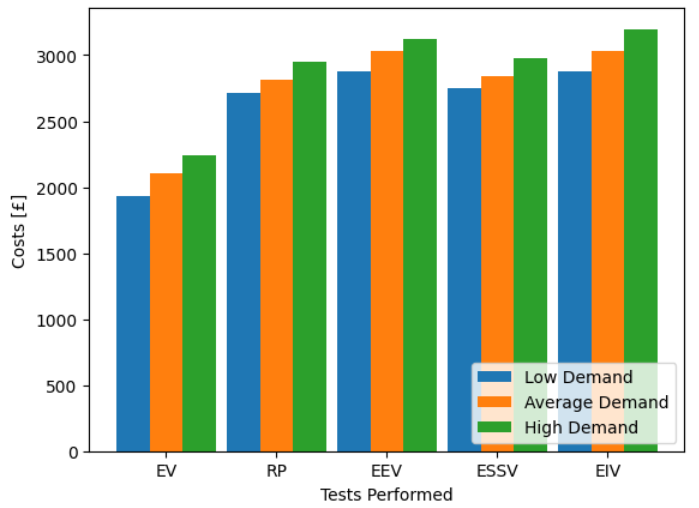
\includegraphics{Chapters/Chapter4New/Figures/WEColumnChart.png}
    \caption{Worked Example Results for the Deterministic and Stochastic Models with Test Results}
    \label{fig:WETests}
\end{figure}

The results show, the deterministic solution does not perform well in a stochastic environment, because of the too low number of beds and staff deployed at the first stage. By performing Test A, this showed that there may be value considering the deterministic solution as a lower bound for the stochastic case. Test B has shown that the deterministic solution performed poorly because it deployed the incorrect number of beds and staffing. Finally, Test C, showed the user that even if some beds and staff are planned using the deterministic model, the stochastic model provides options on how to upgrade or improve the solution. It also informed the user as to where shortages are likely to be expected.

\section{Summary}
Prescriptive analytics offer healthcare professionals the opportunity to optimise outcomes by recommending the best course of action for patients or providers. Often healthcare decisions are made using simple tools or on staff intuition, the results can be less than ideal outcomes and potentially provide unnecessary risks to patients. Using more evidence-based and unbiased approaches, prescriptive analytics can be driven by real-time data which is routinely collected. The impact of selecting different actions can be evaluated prior to implementation, due to the ability to perform numerous scenario analysis.  

This chapter has provided an introduction into two prescriptive methodologies, deterministic and two-stage stochastic modelling. Expanding on the two-stage stochastic programming paradigm and building on the tests introduced by Maggioni and Wallace \cite{Maggioni2010}, this chapter has gone further by creating two-dimensional decision variables which are dependent on each other along with the application to a different field of research, namely healthcare. To demonstrate the procedure and the robustness of the models, a simplified worked example including two hospitals and two specialties was used. The tests discussed in \cite{Maggioni2010}, have also been employed, applied and evaluated to each of the examples.

In the following chapter, Chapter \ref{chp:Experimental Analysis}, the theory from this and the previous chapter will be applied to a case study of frail and elderly patients. The deterministic and two-stage stochastic models developed will be expanded to a case of 14 hospitals and 29 specialties, to determine how to effectively organise bed numbers and staffing requirements to fulfil current and future demands, whilst being mindful of increasing medical costs.
\end{document}  